\documentclass[11pt]{article}
\usepackage[utf8]{inputenc}
\usepackage[T1]{fontenc}
\usepackage{geometry}
\usepackage{graphicx}
\usepackage{booktabs}
\usepackage{float}
\usepackage{amsmath}
\usepackage{array}
\usepackage{longtable}
\usepackage{hyperref}
\usepackage{caption}
\geometry{margin=1in}
\hypersetup{colorlinks=true, linkcolor=black, urlcolor=blue, citecolor=black}

\title{Mahoraga 14.1: consolidaci\'on auditada de un sistema long-only con alpha residualizado, overrides estructurales y continuation lift bajo validaci\'on walk-forward}
\author{Salazar Mart\'inez Liam Antonio}
\date{29 de abril de 2026}

\begin{document}
\maketitle

\section*{Resumen}
Mahoraga 14.1 es una consolidaci\'on auditada de Mahoraga 14 cuyo objetivo no es expandir la arquitectura del sistema, sino verificar que el modo FULL produzca salidas out-of-sample confiables, trazables y consistentes con el modo FAST. La implementaci\'on final conserva tres elementos operativos: un motor base de alpha (\texttt{BASE\_ALPHA\_V2}), una defensa estructural (\texttt{STRUCTURAL\_DEFENSE\_ONLY}) y un m\'odulo de continuation lift (\texttt{CONTINUATION\_PRESSURE\_V2\_ONLY}), adem\'as de una rama combinada con ambos overrides. El trabajo documenta la arquitectura efectiva del c\'odigo, distingue los m\'odulos activos de los descartados, y formaliza la auditor\'ia FULL sobre stitched out-of-sample, recomputaci\'on de \textit{maximum drawdown}, suite de stress y Monte Carlo con dependencia temporal preservada.

En stitched OOS, \texttt{BASE\_ALPHA\_V2} obtiene 24.52\% de CAGR, 1.1887 de Sharpe y -20.24\% de MaxDD, mientras que \texttt{BASE\_ALPHA\_V2 + CONTINUATION\_PRESSURE\_V2\_ONLY} alcanza 24.68\%, 1.1937 y -20.24\%, respectivamente. La mejora directa frente a la base es peque\~na pero real en el stitched agregado ($p=0.033412$), aunque no sobrevive la correcci\'on por multiplicidad disponible en la corrida FULL ($q=1.0$). Por separado, el alpha anualizado con covarianza Newey-West frente a \texttt{QQQ} y \texttt{SPY} permanece positivo y con estad\'isticos $t$ superiores a 2 en la muestra stitched. La auditor\'ia FULL confirma que el stitched concatena exclusivamente ventanas \texttt{TEST\_ONLY}, sin solapes ni huecos, y que el MaxDD reportado coincide exactamente con una recomputaci\'on independiente. La evidencia respalda a Mahoraga 14.1 como una versi\'on metodol\'ogicamente consolidada y apta para an\'alisis t\'ecnico, aunque con l\'imites claros: mejoras incrementales, activaciones de continuation escasas y restricciones de universo derivadas del uso de \textit{LiqSizeProxy} en lugar de FFMC/GICS de verdadera naturaleza point-in-time.

\section{Introducci\'on}
Mahoraga es un sistema long-only sobre un universo concentrado de emisores tecnol\'ogicos y de plataforma cuyo objetivo operativo es producir una trayectoria out-of-sample superior a una base hist\'orica interna (\texttt{LEGACY}), y competitiva frente a \texttt{QQQ} y \texttt{SPY}, sin abandonar trazabilidad del pipeline ni interpretabilidad de las decisiones. En Mahoraga 14.1, ese objetivo se redefine con una restricci\'on adicional: antes de extraer conclusiones econ\'omicas, el modo FULL debe demostrar integridad metodol\'ogica en stitched OOS, drawdown, stress testing y Monte Carlo.

Esta exigencia no es ret\'orica. El proyecto arrastraba dos riesgos hist\'oricos concretos: un stitched OOS mal armado que contaminaba la lectura out-of-sample, y episodios donde stitched o stress inflaban artificialmente el MaxDD. Por ello, Mahoraga 14.1 debe leerse como una consolidaci\'on auditada antes que como una versi\'on expansiva. La pregunta central es doble: qu\'e sobrevive realmente en la implementaci\'on final, y cu\'al es la evidencia emp\'irica que sigue siendo defendible una vez auditado el pipeline FULL.

\section{Evoluci\'on del proyecto y antecedentes de investigaci\'on}
La base hist\'orica del proyecto permanece preservada en \texttt{mahoraga6\_1.py}, mientras que el paquete \texttt{mahoraga14/} modulariza la l\'ogica en componentes separados de datos, motor de alpha, overrides, ejecuci\'on de backtest y reporte. La documentaci\'on interna explicita dos decisiones arquitect\'onicas relevantes: no existe capa Markov y la se\~nal Hawkes se utiliza s\'olo como se\~nal r\'apida de transici\'on, no como un modelo puntual completamente estimado.

La consolidaci\'on 14.1 mantiene cinco hip\'otesis previas y descarta otras. Sobreviven: (i) \texttt{BASE\_ALPHA\_V2} como base fuerte; (ii) \texttt{CONTINUATION\_PRESSURE\_V2\_ONLY} como mejora stitched peque\~na pero real; (iii) \texttt{STRUCTURAL\_DEFENSE\_ONLY} como m\'odulo de apoyo al suelo, no como rama principal; (iv) alpha benchmark-adjusted positivo frente a \texttt{QQQ} y \texttt{SPY}; y (v) necesidad de auditor\'ia completa antes de interpretar FULL. En cambio, quedan fuera de la descripci\'on final del sistema los clasificadores standalone de transici\'on/recuperaci\'on, la capa Markov, el \textit{ML RegimeGate} hist\'orico, cualquier rama long-short y cualquier m\'odulo de deep learning o reinforcement learning. Tambi\'en se descarta el FULL como motor de descubrimiento combinatorio amplio: en 14.1 se convierte en un modo de auditor\'ia dirigido, con la misma malla focalizada que FAST.

Desde el punto de vista metodol\'ogico, las piezas que s\'i tienen apoyo expl\'icito en la implementaci\'on se apoyan en referencias conocidas pero usadas de forma acotada: covarianza HAC de Newey y West para alpha frente a benchmark, \textit{hierarchical risk parity} para el reparto intracartera, regularizaci\'on ridge en la residualizaci\'on y clasificadores log\'isticos / \textit{random forest} como retadores sencillos y auditables \cite{NeweyWest1987, LopezdePrado2016, HoerlKennard1970, Breiman2001}. La analog\'ia Hawkes se conserva s\'olo a nivel de intensidades deca\'idas de eventos de estr\'es y recuperaci\'on \cite{Hawkes1971}.

\section{Datos, universo y preparaci\'on de informaci\'on}
La configuraci\'on auditada cubre datos diarios entre 2005-01-01 y 2026-02-20, con capital inicial de 100{,}000 unidades monetarias y decisi\'on semanal en cierres de viernes. El pipeline consume series OHLCV para el universo operativo y para los benchmarks \texttt{QQQ}, \texttt{SPY} y, cuando est\'a disponible, \texttt{VIX}. En el cargado de datos tambi\'en se recuperan factores FF, pero la capa FULL auditada de Mahoraga 14.1 no utiliza esa informaci\'on en sus salidas operativas; por ello no se presenta aqu\'i como componente activo del sistema final.

El universo auditado es un universo can\'onico reconstituido trimestralmente con una variable de ranking denominada \textit{LiqSizeProxy}, definida como el promedio de precio por volumen sobre 30 d\'ias. El motor de universo usa tama\~no objetivo 10, autoentrada hasta rank 8, retenci\'on hasta rank 10, buffer hasta rank 13, estacionalidad m\'inima de 63 d\'ias y volumen d\'olar promedio m\'inimo de USD 50 millones. La propia base hist\'orica del proyecto explicita que este mecanismo no es FFMC ni clasificaci\'on GICS-IT real; para ello har\'ian falta datos CRSP/Compustat point-in-time que no forman parte de la implementaci\'on auditada. En consecuencia, Mahoraga 14.1 reduce, pero no elimina plenamente, los riesgos de sesgo de supervivencia y de clasificaci\'on ex post.

La preparaci\'on de informaci\'on opera en dos escalas. En frecuencia diaria se construyen scores, pesos, stops, escalados de riesgo, costos y benchmarks. En frecuencia semanal se genera un \textit{dataset} de trayectoria y contexto de mercado que alimenta a la defensa estructural, a continuation y a la se\~nal Hawkes-style. Esta separaci\'on es importante: los overrides se calibran semanalmente, pero su efecto se traslada a ejecuci\'on diaria mediante un mapeo semanal-a-diario auditado.

\section{Arquitectura del sistema}
La arquitectura final de Mahoraga 14.1 puede describirse en cuatro capas. La primera es un motor base de alpha que produce pesos objetivo y una trayectoria base (\texttt{BASE\_ALPHA\_V2}). La segunda es una trayectoria defensiva precomputada con el mismo conjunto de componentes de alpha, pero con distinta mezcla de score y penalizaci\'on de beta. La tercera es una capa superior de overrides semanales que decide, en cada fecha de decisi\'on, si conviene activar defensa estructural o continuation lift. La cuarta es la capa de auditor\'ia FULL, implementada en \texttt{full\_report.py}, que reconstruye stitched OOS, verifica integridad temporal, recompone equity y drawdown, ejecuta stress tests y produce Monte Carlo con dependencia temporal preservada.

La ruta de ejecuci\'on efectiva es estricta: \texttt{mahoraga14\_runner.py} crea la configuraci\'on; \texttt{mahoraga14\_data.py} carga datos y universo; \texttt{backtest\_executor.py} corre el walk-forward y ensambla las variantes; \texttt{full\_report.py} construye la salida FULL auditada. Esa ruta no llama a los clasificadores standalone de transici\'on/recuperaci\'on, y por lo tanto dichos m\'odulos no deben interpretarse como parte activa de Mahoraga 14.1, aunque sigan presentes en el repositorio como referencia hist\'orica.

\section{Metodolog\'ia}
La metodolog\'ia de Mahoraga 14.1 combina calibraci\'on dirigida y auditor\'ia posterior. El modo FAST y el modo FULL comparten la misma malla focalizada de hiperpar\'ametros. Esta decisi\'on es expl\'icita en configuraci\'on: FULL deja de ser una b\'usqueda combinatoria abierta y se restringe a la misma cuadr\'icula de \texttt{base\_mix}, \texttt{defense\_mix}, penalizaciones de beta y \texttt{raw\_rel\_boost} usada por FAST. El objetivo es preservar comparabilidad entre ambos modos y evitar que FULL se convierta en una fuente adicional de sobreajuste o en un proceso computacional explosivo.

La comparaci\'on emp\'irica se organiza alrededor de tres candidatos auditados: \texttt{BASE\_ALPHA\_V2}, \texttt{BASE\_ALPHA\_V2 + CONTINUATION\_PRESSURE\_V2\_ONLY} y \texttt{BASE\_ALPHA\_V2 + STRUCTURAL\_DEFENSE\_ONLY + CONTINUATION\_PRESSURE\_V2}. \texttt{STRUCTURAL\_DEFENSE\_ONLY} se conserva como referencia auxiliar. Los benchmarks obligatorios son \texttt{LEGACY}, \texttt{QQQ} y \texttt{SPY}. Las pruebas directas de comparaci\'on usan $p$-values emparejados sobre retornos de ventana y su ajuste BHY disponible en el pipeline. El alpha ajustado por benchmark se estima mediante una regresi\'on
\begin{equation}
r^{(s)}_t = \alpha + \beta r^{(b)}_t + \varepsilon_t,
\end{equation}
con covarianza HAC Newey-West y anualizaci\'on del intercepto \cite{NeweyWest1987}. Esta distinci\'on es central en la lectura de resultados: un alpha positivo frente a benchmark no es equivalente a una mejora estad\'isticamente s\'olida frente a la base interna despu\'es de correcci\'on por multiplicidad.

\section{Construcci\'on del motor de alpha}
El motor \texttt{BASE\_ALPHA\_V2} mezcla un \textit{core} legado con una capa adaptiva residualizada. El \textit{core} legado se compone de tres bloques: tendencia, momentum y momentum relativo contra \texttt{QQQ}. En paralelo, la capa adaptiva construye un score en precios brutos y otro en precios residualizados frente a cuatro factores: \texttt{QQQ}, \texttt{SPY}, un factor \texttt{TECH} definido como retorno medio transversal del universo y el primer componente principal (\texttt{PC1}) de los retornos de entrenamiento.

La residualizaci\'on se estima por activos mediante regresi\'on ridge rodante con ventana de 63 observaciones, m\'inimo de 42 observaciones, $\alpha=8.0$ y recorte de retornos residualizados a $\pm 0.25$. Sobre la trayectoria residualizada se recomputan se\~nales de tendencia y momentum. Los pesos del bloque bruto se aprenden con IC transversal y luego se contraen hacia un prior uniforme $(1/3,1/3,1/3)$ con \texttt{raw\_weight\_shrink}=0.70; los pesos del bloque residualizado se contraen hacia $(0.5,0.5)$ con \texttt{resid\_weight\_shrink}=0.60. El score diario final sigue la forma
\begin{align}
\text{legacy\_core}_{i,t} &= z\!\left(w_{tr}\,\text{legacy\_tr}_{i,t} + w_{mo}\,\text{legacy\_mo}_{i,t} + w_{re}\,\text{legacy\_re}_{i,t}\right), \\
\text{raw\_score}_{i,t} &= w^{raw}_1 \,\text{raw\_tr}_{i,t} + w^{raw}_2 \,\text{raw\_mo}_{i,t} + w^{raw}_3 \,\text{raw\_re}_{i,t}, \\
\text{resid\_score}_{i,t} &= w^{res}_1 \,\text{resid\_tr}_{i,t} + w^{res}_2 \,\text{resid\_mo}_{i,t}, \\
\text{adaptive\_score}_{i,t} &= 0.62\,\text{raw\_score}_{i,t} + 0.38\,\text{resid\_score}_{i,t} - \text{beta\_drag}_{i,t}, \\
\text{score}_{i,t} &= z\!\left((1-m)\,\text{legacy\_core}_{i,t} + m\,\text{adaptive\_score}_{i,t}\right).
\end{align}

El t\'ermino \texttt{beta\_drag} penaliza exposiciones con beta superior a 1.0. El score se anula durante el \textit{burn-in} inicial, definido como el m\'aximo entre 252 d\'ias y el \textit{burn-in} residual de 126 d\'ias. En t\'erminos funcionales, el motor base persigue una combinaci\'on de persistencia direccional, momentum relativo y depuraci\'on parcial del movimiento de benchmark.

\section{Construcci\'on de cartera y ejecuci\'on}
En cada fecha de rebalanceo semanal se seleccionan hasta tres nombres con score positivo. Si s\'olo hay un nombre elegible, se asigna peso unitario; si hay dos o m\'as, se utiliza \textit{hierarchical risk parity} (HRP) sobre una ventana de 252 d\'ias, con retroceso a historial completo si la ventana reciente es insuficiente, y con tope de peso individual de 60\% \cite{LopezdePrado2016}. Si no hay nombres elegibles, la cartera permanece en efectivo.

Los pesos objetivo pasan por un \textit{Chandelier stop} antes de ejecutarse. Los pesos ejecutados quedan desplazados un d\'ia (\texttt{shift(1)}), con lo que la simulaci\'on evita ejecutar el mismo d\'ia en que se observa el score o se activa el stop. La serie de retornos brutos se obtiene como producto entre pesos ejecutados y retornos diarios del universo. La ejecuci\'on neta deduce costos proporcionales al turnover; en la configuraci\'on base auditada, la comisi\'on es 10 bps y el slippage 3 bps.

La reconstrucci\'on de equity responde a la expresi\'on
\begin{equation}
E_t = E_0 \prod_{s \le t}(1 + r^{net}_s),
\end{equation}
con $E_0=100{,}000$. Esta definici\'on se usa de manera uniforme en backtest, stitched, stress suite y auditor\'ia de MaxDD. El benchmark \texttt{QQQ} descuenta adem\'as un costo anual de gastos del ETF, mientras que \texttt{SPY} se usa sobre retorno simple diario.

\section{Gesti\'on de riesgo y reglas de salida}
La gesti\'on de riesgo se implementa por capas. Primero se estima una volatilidad realizada sobre 63 d\'ias y se compara con una volatilidad objetivo anual de 30\%. Luego se impone un cap multiplicativo formado por \texttt{crisis\_scale}, \texttt{turb\_scale}, un veto secundario de correlaci\'on y, en caso de override, los multiplicadores \texttt{gate\_scale} y \texttt{exp\_cap}. Si la correlaci\'on media cruza 0.90, el veto secundario escala la exposici\'on a 0.80. La exposici\'on final efectiva corresponde al m\'inimo entre escala por volatilidad y cap agregado, y tambi\'en se desplaza un d\'ia antes de aplicarse.

Las reglas de salida forman parte de la propia construcci\'on de pesos y del bloque de overrides. En la ruta base, los \textit{stops} liberan la posici\'on. En la ruta estructural, el sistema puede forzar una mezcla parcial hacia la trayectoria defensiva y reducir techo de exposici\'on. En la ruta continuation, el sistema no reemplaza la cartera base; s\'olo relaja ligeramente los topes de escala cuando la se\~nal de continuation supera umbrales de activaci\'on y mantiene bajo el riesgo de ruptura.

El drawdown se define de forma can\'onica como
\begin{equation}
DD_t = \frac{E_t}{\max_{s \le t} E_s} - 1.
\end{equation}
Esta misma definici\'on se reutiliza en la auditor\'ia FULL para evitar discrepancias entre drawdown reportado y equity reconstruida.

\section{Overrides y capa superior}
La capa superior contiene dos m\'odulos activos. El primero es la defensa estructural. A partir de un \textit{dataset} semanal con informaci\'on de drawdown, duraci\'on de drawdown, velocidad, rebote, eficiencia, share de p\'erdidas, densidad de stops, persistencia de correlaci\'on, amplitud transversal, drawdown de \texttt{QQQ}, \texttt{VIX} y escalas de crisis/turbulencia/correlaci\'on, se construye una etiqueta \texttt{structural\_y} asociada a retornos futuros bajos, empeoramiento del drawdown y debilidad relativa. El modelo estructural elige entre un clasificador log\'istico estandarizado y un \textit{random forest} retador, qued\'andose con el que maximiza AUC de validaci\'on.

La probabilidad \texttt{structural\_p} no act\'ua sola. El score semanal de defensa se define como
\begin{equation}
\text{structural\_score} = 0.74\,\text{structural\_p} + 0.22\,\text{structural\_path} + 0.04\,w_H\,\text{stress\_hawkes},
\end{equation}
donde \texttt{structural\_path} resume la geometr\'ia reciente del drawdown y \texttt{stress\_hawkes} es la intensidad Hawkes-style de estr\'es. Si el score supera el umbral calibrado y se cumplen guardas adicionales de deterioro de trayectoria, la capa superior activa \texttt{STRUCTURAL\_DEFENSE}: mezcla parcialmente la trayectoria base con una trayectoria defensiva precomputada y reduce \texttt{gate\_scale}, \texttt{vol\_mult} y \texttt{exp\_cap}.

El segundo m\'odulo activo es \texttt{CONTINUATION\_PRESSURE\_V2}. Su dise\~no est\'a separado en tres subproblemas: \textit{trigger}, \textit{pressure} y \textit{break-risk}. Las caracter\'isticas de \textit{trigger} enfatizan liberaci\'on de stops, rebotes de amplitud y estados de compresi\'on; las de \textit{pressure} miden eficiencia de trayectoria, amplitud de swings, retornos recientes y relaci\'on frente a \texttt{QQQ}; las de \textit{break-risk} combinan esos elementos con riesgo de estr\'es Hawkes-style. Cada submodelo elige entre log\'istica y \textit{random forest} seg\'un AUC de validaci\'on. Los scores principales son
\begin{align}
\text{trigger\_score} &= 0.65\,\text{trigger\_p} + 0.35\,\text{trigger\_context}, \\
\text{pressure\_score} &= 0.60\,\text{pressure\_p} + 0.40\,\text{pressure\_context}.
\end{align}

La activaci\'on de continuation exige que la defensa estructural no est\'e activa, que exista compresi\'on o pausa v\'alida, apoyo de benchmark, alguna se\~nal gatillo de liberaci\'on o rebote, score estructural suficientemente bajo y probabilidad de \textit{break-risk} por debajo de un cap calibrado. Si se cumple esa combinaci\'on, el sistema activa \texttt{CONTINUATION\_LIFT}. Es importante subrayar que continuation no construye una cartera nueva: mantiene \texttt{defense\_blend}=0 y s\'olo relaja moderadamente \texttt{gate\_scale}, \texttt{vol\_mult} y \texttt{exp\_cap} en proporci\'on a una intensidad suave de continuation. En este sentido, continuation es una capa de exposici\'on, no un motor de alpha alternativo.

El rol de Hawkes en esta secci\'on debe interpretarse de forma literal. La implementaci\'on final no estima un proceso Hawkes multivariante. En cambio, define eventos de estr\'es y recuperaci\'on y propaga intensidades por la recurrencia
\begin{equation}
\lambda_t = \delta \lambda_{t-1} + I_{t-1},
\end{equation}
con $\delta=0.70$ y recorte posterior de la intensidad. Por ello, el t\'ermino correcto para el paper es \textit{se\~nal Hawkes-style} o \textit{Hawkes-inspired}, no \textit{modelo Hawkes estimado}.

\section{Backtesting y protocolo walk-forward}
El backtest se organiza en cinco folds expandentes con embargo expl\'icito de 252 d\'ias entre fin de entrenamiento y comienzo de validaci\'on. Las ventanas son: (i) entrenamiento hasta 2013-12-31, validaci\'on 2015-01-02 a 2016-12-30 y test 2017-01-03 a 2018-12-31; (ii) entrenamiento hasta 2015-12-31, validaci\'on 2017-01-03 a 2018-12-31 y test 2019-01-02 a 2020-12-31; (iii) entrenamiento hasta 2017-12-29, validaci\'on 2019-01-02 a 2020-12-31 y test 2021-01-04 a 2022-12-30; (iv) entrenamiento hasta 2019-12-31, validaci\'on 2021-01-04 a 2022-12-30 y test 2023-01-03 a 2024-06-28; y (v) entrenamiento hasta 2021-12-31, validaci\'on 2023-01-03 a 2024-06-28 y test 2024-07-01 a 2026-02-20.

La selecci\'on de hiperpar\'ametros durante calibraci\'on sigue una l\'ogica heredada de Mahoraga 14: la malla principal se organiza alrededor de \texttt{STRUCTURAL\_DEFENSE\_ONLY} como \texttt{main\_variant\_key}. Sin embargo, la capa FULL auditada en 14.1 fija \texttt{CONTINUATION\_PRESSURE\_V2\_ONLY} como \texttt{full\_primary\_variant\_key}. Este detalle no es un bug, sino una decisi\'on de consolidaci\'on: la calibraci\'on conserva comparabilidad con FAST, mientras que la auditor\'ia final se centra en la rama continuation, que es la mejora stitched m\'as defendible sobre la base.

\section{Auditor\'ia FULL: stitched, MaxDD, stress tests y Monte Carlo}
\subsection*{Stitched OOS}
La auditor\'ia stitched produce una traza por fold (\texttt{stitched\_full\_trace.csv}) y un conjunto de chequeos de integridad (\texttt{stitched\_integrity\_checks.csv}). Para todas las variantes y benchmarks auditados, la concatenaci\'on utiliza exclusivamente ventanas \texttt{TEST\_ONLY} con filas por segmento [502, 505, 503, 374, 411], sin solapes y sin huecos. Los \'indices stitched son mon\'otonos, \'unicos y coinciden con el calendario OOS efectivo esperado. La reconstrucci\'on de exposici\'on, turnover y costos tambi\'en pasa verificaci\'on.

El \'unico chequeo informativo que no es estrictamente verdadero en sentido nominal es \texttt{requested\_bounds\_fully\_available}: el fold 5 se pide hasta 2026-02-20, pero el calendario efectivo realizable termina en 2026-02-19. La traza expone esta diferencia de forma expl\'icita y la clasificaci\'on final permanece en PASS porque la concatenaci\'on coincide con el calendario OOS efectivamente disponible. Esta es una diferencia importante frente a errores hist\'oricos: el l\'imite efectivo se declara, no se oculta.

\subsection*{Auditor\'ia de MaxDD}
La auditor\'ia de drawdown reconstruye la equity stitched desde retornos netos diarios, calcula el \textit{running peak} y recompone el drawdown con la misma definici\'on usada en el backtest. Los resultados se guardan en \texttt{maxdd\_audit\_full.csv} y \texttt{maxdd\_audit\_notes.md}. En todas las variantes y benchmarks, el MaxDD almacenado coincide exactamente con el MaxDD reconstruido; la diferencia auditada es 0.0 puntos base. Para la base y el candidato continuation, el episodio m\'aximo stitched se localiza entre el pico del 2020-09-01 y el trough del 2020-11-10, con recuperaci\'on el 2021-07-23. Por lo tanto, el MaxDD reportado en FULL no proviene de una recomposici\'on defectuosa del stitched.

\subsection*{Stress suite}
La suite de stress auditada incluye aumentos de costos (+25\%, +50\%, +100\%), slippage adicional, delay de un rebalance, falsos positivos extra en continuation, falsos positivos extra en structural defense, reducci\'on del continuation lift, stress conjunto de \texttt{gate\_scale}/\texttt{vol\_mult}/\texttt{exp\_cap} y un \textit{empirical tail block path stress}. Seg\'un \texttt{stress\_suite\_audit.md}, todos los escenarios no basados en trayectoria recomputan retornos, equity, drawdown y alpha desde las mismas ventanas stitched \texttt{TEST\_ONLY}; los benchmarks mantienen sus trayectorias base para comparaci\'on.

El \textit{empirical tail block path stress} reemplaza bloques de retornos por episodios emp\'iricos de cola ya observados, preservando estructura temporal a nivel de bloque. Esta decisi\'on es metodol\'ogicamente m\'as consistente con el objetivo de auditor\'ia que una perturbaci\'on IID. Sin embargo, la suite debe interpretarse como an\'alisis de sensibilidad, no como garant\'ia de que todo stress empeora todas las m\'etricas. De hecho, algunos escenarios de falsos positivos estructurales mejoran marginalmente la muestra del combo y de la rama estructural, lo cual se documenta de forma expl\'icita en los resultados y no se fuerza a interpretaci\'on adversa.

\subsection*{Monte Carlo y bootstrap}
Mahoraga 14.1 incorpora tres herramientas de robustez. La primera es un \textit{stationary block bootstrap} sobre retornos stitched \texttt{TEST\_ONLY}, que preserva dependencia temporal local. La segunda es un Monte Carlo de fricciones que multiplica la serie de costos realizada. La tercera es una perturbaci\'on local de par\'ametros alrededor del candidato final continuation. No se incluye Monte Carlo IID ingenuo, precisamente para evitar destruir la estructura temporal del proceso.

Las salidas relevantes son \texttt{montecarlo\_summary\_full.csv}, \texttt{montecarlo\_percentiles\_full.csv} y \texttt{montecarlo\_audit.md}. El bootstrap estacionario es la pieza m\'as informativa: para el candidato primario arroja mediana de CAGR de 24.27\%, mediana de Sharpe de 1.1959 y mediana de MaxDD de -24.36\%, con probabilidad de 28.5\% de caer por debajo de Sharpe 1 y de 44.75\% de registrar un MaxDD inferior a -25\%. La simulaci\'on de fricciones y la vecindad local muestran dispersi\'on mucho menor, como es esperable dado que exploran perturbaciones m\'as acotadas.

\section{Resultados}
La Tabla \ref{tab:stitched-key-results} resume el stitched OOS final. La base fuerte del sistema es \texttt{BASE\_ALPHA\_V2}, con 24.52\% de CAGR, 1.1887 de Sharpe y -20.24\% de MaxDD. Frente a esta base, la rama continuation produce 24.68\%, 1.1937 y -20.24\%, mientras que la rama combinada produce 24.57\%, 1.1912 y -20.27\%. La rama puramente estructural queda en 24.41\%, 1.1862 y -20.27\%. Frente a benchmarks, el candidato continuation supera a \texttt{LEGACY}, \texttt{QQQ} y \texttt{SPY} tanto en CAGR como en Sharpe y MaxDD stitched.

\begin{table}[H]
\centering
\caption{Comparacion stitched OOS FULL de los candidatos auditados y benchmarks obligatorios. El alpha Newey-West se reporta en terminos anualizados frente a \texttt{QQQ} y \texttt{SPY}.}
\label{tab:stitched-key-results}
\resizebox{\textwidth}{!}{%
\begin{tabular}{lrrrrrrr}
\toprule
Variante & CAGR (\%) & Sharpe & MaxDD (\%) & Exposicion media & Turnover medio & AlphaNW QQQ & AlphaNW SPY \\
\midrule
LEGACY & 23.07 & 1.1348 & -21.11 & 0.6069 & 0.0331 & 0.1400 & 0.1729 \\
QQQ & 20.14 & 0.9178 & -35.24 & 1.0000 & 0.0000 & 0.0000 & 0.0294 \\
SPY & 14.88 & 0.8463 & -33.72 & 1.0000 & 0.0000 & -0.0021 & 0.0000 \\
BASE\_ALPHA\_V2 & 24.52 & 1.1887 & -20.24 & 0.6303 & 0.0345 & 0.1479 & 0.1814 \\
BASE + CONTINUATION\_PRESSURE\_V2\_ONLY & 24.68 & 1.1937 & -20.24 & 0.6316 & 0.0345 & 0.1494 & 0.1830 \\
BASE + STRUCTURAL\_DEFENSE\_ONLY + CONTINUATION\_PRESSURE\_V2 & 24.57 & 1.1912 & -20.27 & 0.6269 & 0.0342 & 0.1498 & 0.1832 \\
BASE + STRUCTURAL\_DEFENSE\_ONLY & 24.41 & 1.1862 & -20.27 & 0.6256 & 0.0342 & 0.1484 & 0.1817 \\
\bottomrule
\end{tabular}}
\end{table}


La lectura estad\'istica requiere separar dos niveles. Primero, la mejora directa continuation vs.\ base tiene un $p$-value stitched de 0.033412, coherente con una mejora peque\~na pero real. Segundo, el ajuste BHY disponible en la corrida devuelve $q=1.0$, de modo que esa evidencia no debe presentarse como una ganancia robusta bajo control estricto de multiplicidad. En paralelo, el alpha anualizado Newey-West stitched del candidato continuation es 0.1494 frente a \texttt{QQQ} ($t=2.490$) y 0.1830 frente a \texttt{SPY} ($t=2.716$). As\'i, el benchmark-adjusted alpha sigue siendo positivo y estad\'isticamente m\'as convincente que la comparaci\'on directa corregida frente a la base.

La Tabla \ref{tab:floor-ceiling-selection} resume la jerarqu\'ia de ramas. \texttt{STRUCTURAL\_DEFENSE\_ONLY} mejora modestamente el suelo promedio (0.5392 vs.\ 0.5291 de Sharpe en folds de piso), pero no supera a la base en stitched total y queda clasificada como \texttt{MAIN\_BRANCH\_FAIL}. \texttt{CONTINUATION\_PRESSURE\_V2\_ONLY} mejora techo, suelo y stitched, pero carga la nota \texttt{fold3\_below\_main}; aun as\'i, en 14.1 se adopta como candidato primario porque su mejora stitched es la m\'as n\'itida y consistente con el objetivo de auditor\'ia. La rama combinada pasa filtros, pero sin un perfil suficientemente superior como para desplazar a continuation.

\begin{table}[H]
\centering
\caption{Resumen de piso/techo y estatus de seleccion de las ramas auditadas. La defensa estructural mejora modestamente los folds de suelo, pero no supera a la base en stitched agregado.}
\label{tab:floor-ceiling-selection}
\resizebox{\textwidth}{!}{%
\begin{tabular}{lrrrrrrl}
\toprule
Variante & Ceiling Sharpe & Delta ceiling & Floor Sharpe & Delta floor & Stitched Sharpe & Delta stitched & Estatus \\
\midrule
BASE\_ALPHA\_V2 & 1.5523 & 0.0000 & 0.5291 & 0.0000 & 1.1887 & 0.0000 & OFFICIAL\_BASELINE \\
BASE + STRUCTURAL\_DEFENSE\_ONLY & 1.5378 & -0.0146 & 0.5392 & 0.0101 & 1.1862 & -0.0025 & MAIN\_BRANCH\_FAIL \\
BASE + CONTINUATION\_PRESSURE\_V2\_ONLY & 1.5589 & 0.0066 & 0.5310 & 0.0019 & 1.1937 & 0.0050 & REJECT \\
BASE + STRUCTURAL\_DEFENSE\_ONLY + CONTINUATION\_PRESSURE\_V2 & 1.5444 & -0.0080 & 0.5411 & 0.0120 & 1.1912 & 0.0025 & PASS\_NOT\_PROMISING \\
\bottomrule
\end{tabular}}
\end{table}


La utilizaci\'on efectiva de los overrides tambi\'en es informativa. En stitched, continuation registra una tasa de lift de 5.19\% y una tasa de activaci\'on de 2.10\%, lo que confirma que se trata de una intervenci\'on escasa y selectiva. El event study stitched sobre 10 activaciones muestra retornos medios posteriores de 0.69\% a 1 semana, 3.28\% a 2 semanas y 6.26\% a 4 semanas, frente a 1.88\% a 4 semanas en no activaciones. Esta evidencia es descriptiva y consistente con la hip\'otesis del m\'odulo, pero su tama\~no muestral obliga a prudencia interpretativa.

\begin{table}[H]
\centering
\caption{Event study stitched de activaciones de continuation para el candidato primario. La muestra es pequena y debe interpretarse como evidencia descriptiva auxiliar.}
\label{tab:continuation-event-study}
\begin{tabular}{lrrrrrr}
\toprule
Variante & Activaciones & Hit rate & Retorno medio 1W & Retorno medio 2W & Retorno medio 4W & Drawdown medio 4W \\
\midrule
Activacion continuation & 10 & 0.5833 & 0.0069 & 0.0328 & 0.0626 & -0.0066 \\
No activacion & 466 & 0.5258 & 0.0043 & 0.0090 & 0.0188 & -0.0260 \\
\bottomrule
\end{tabular}
\end{table}


En calibraci\'on, los submodelos de continuation muestran AUCs razonables pero heterog\'eneos por fold. El AUC del \textit{trigger} oscila aproximadamente entre 0.67 y 0.87; el de \textit{pressure}, entre 0.58 y 0.79; y el de \textit{break-risk}, entre 0.76 y 0.80. Estos valores respaldan que continuation no es una regla puramente ad hoc, pero tambi\'en confirman que la se\~nal no es uniformemente fuerte en todos los reg\'imenes.

La auditor\'ia de stitched y MaxDD se resume en la Tabla \ref{tab:audit-integrity-maxdd}. La igualdad entre MaxDD almacenado y recomputado descarta el tipo de contaminaci\'on que motiv\'o Mahoraga 14.1. En otras palabras, la mejora continuation no descansa en una construcci\'on defectuosa de equity o drawdown.

\begin{table}[H]
\centering
\caption{Resumen de auditoria FULL para stitched y MaxDD. Todas las variantes pasan integridad de stitched, reconstruccion de equity y recomputacion independiente de drawdown.}
\label{tab:audit-integrity-maxdd}
\begin{tabular}{lccc}
\toprule
Chequeo & Resultado & Detalle principal & Implicacion \\
\midrule
Ventanas stitched & PASS & solo segmentos TEST\_ONLY & no hay contaminacion de train/val \\
Traza por fold & PASS & filas [502, 505, 503, 374, 411] & sin perdidas de observaciones \\
Overlap / gaps & PASS & overlap=False; gap=0 por fold & concatenacion contigua \\
Indices temporales & PASS & monotonicidad e indices unicos & calendario stitched valido \\
Equity reconstruible & PASS & max\_abs\_diff = 0 & equity final consistente \\
Drawdown reconstruible & PASS & drawdown desde equity stitched & sin recomposicion por piezas \\
MaxDD audit & PASS & diff = 0.0 bps & MaxDD no artefactual \\
Disponibilidad nominal fold 5 & INFO & pedido 2026-02-20; efectivo 2026-02-19 & diferencia explicita, no error de stitched \\
\bottomrule
\end{tabular}
\end{table}


La sensibilidad del candidato primario se muestra en la Tabla \ref{tab:stress-primary}. El mayor deterioro de Sharpe proviene del \textit{empirical tail block path stress} (1.0255) y del doblado de costos (1.1378), mientras que el peor MaxDD aparece bajo delay de ejecuci\'on (-20.56\%) o continuation false positives extra (-20.68\%). El stress de \texttt{gate/vol/cap} reduce CAGR, pero mejora el MaxDD hacia -18.59\%, recordando que no todos los stresses representan da\~nos unidireccionales: algunos miden el costo de ser m\'as conservador.

\begin{table}[H]
\centering
\caption{Stress suite del candidato primario \texttt{BASE\_ALPHA\_V2 + CONTINUATION\_PRESSURE\_V2\_ONLY}. Los escenarios recalculan retornos, equity, drawdown y alpha sobre la misma serie stitched \texttt{TEST\_ONLY}.}
\label{tab:stress-primary}
\resizebox{\textwidth}{!}{%
\begin{tabular}{lrrrrr}
\toprule
Escenario & CAGR (\%) & Sharpe & MaxDD (\%) & AlphaNW QQQ & AlphaNW SPY \\
\midrule
Baseline & 24.68 & 1.1937 & -20.24 & 0.1494 & 0.1830 \\
Costos +25\% & 24.33 & 1.1798 & -20.27 & 0.1461 & 0.1796 \\
Costos +50\% & 23.98 & 1.1658 & -20.30 & 0.1429 & 0.1763 \\
Costos +100\% & 23.28 & 1.1378 & -20.37 & 0.1365 & 0.1697 \\
Slippage +5 bps & 24.14 & 1.1722 & -20.29 & 0.1444 & 0.1778 \\
Delay 1 rebalance & 24.34 & 1.1435 & -20.56 & 0.1356 & 0.1684 \\
False positives continuation & 24.67 & 1.1898 & -20.68 & 0.1490 & 0.1828 \\
Continuation lift -50\% & 24.61 & 1.1913 & -20.24 & 0.1487 & 0.1823 \\
Stress gate/vol/cap & 21.54 & 1.2000 & -18.59 & 0.1301 & 0.1587 \\
Empirical tail block path stress & 20.96 & 1.0255 & -20.24 & 0.1167 & 0.1492 \\
\bottomrule
\end{tabular}}
\end{table}


La robustez por simulaci\'on aparece en la Tabla \ref{tab:mc-primary}. El stationary bootstrap mantiene una mediana cercana al stitched observado, pero revela dispersi\'on significativa en drawdown: el percentil 5 del MaxDD para continuation cae a -36.88\%. Esta cola no invalida la muestra base, pero obliga a reconocer que una trayectoria stitched favorable no elimina riesgo de deterioro severo bajo remuestreo por bloques.

\begin{table}[H]
\centering
\caption{Monte Carlo y bootstrap del candidato primario. El bloque estacionario preserva dependencia temporal; la simulacion de fricciones y la perturbacion local se restringen a la implementacion final auditada.}
\label{tab:mc-primary}
\resizebox{\textwidth}{!}{%
\begin{tabular}{lrrrrrr}
\toprule
Metodo & Muestras & Media CAGR (\%) & Media Sharpe & Media MaxDD (\%) & $\Pr(\text{Sharpe}<1)$ & $\Pr(\text{MaxDD}<-25\%)$ \\
\midrule
Stationary block bootstrap & 400 & 24.84 & 1.1909 & -25.36 & 0.2850 & 0.4475 \\
Friction multiplier MC & 300 & 24.68 & 1.1935 & -20.24 & 0.0000 & 0.0000 \\
Local parameter neighborhood & 18 & 24.66 & 1.1929 & -20.24 & 0.0000 & 0.0000 \\
\bottomrule
\end{tabular}}
\end{table}


Las figuras auditadas complementan estas tablas. La Figura \ref{fig:equity} muestra la trayectoria stitched comparada con \texttt{LEGACY}, \texttt{QQQ} y \texttt{SPY}. La Figura \ref{fig:drawdown} permite verificar que la mejora frente a benchmarks no proviene de esconder drawdowns. La Figura \ref{fig:heatmap} resume heterogeneidad por fold, la Figura \ref{fig:contstudy} presenta el event study de continuation y la Figura \ref{fig:mc} la distribuci\'on Monte Carlo.

\begin{figure}[H]
\centering
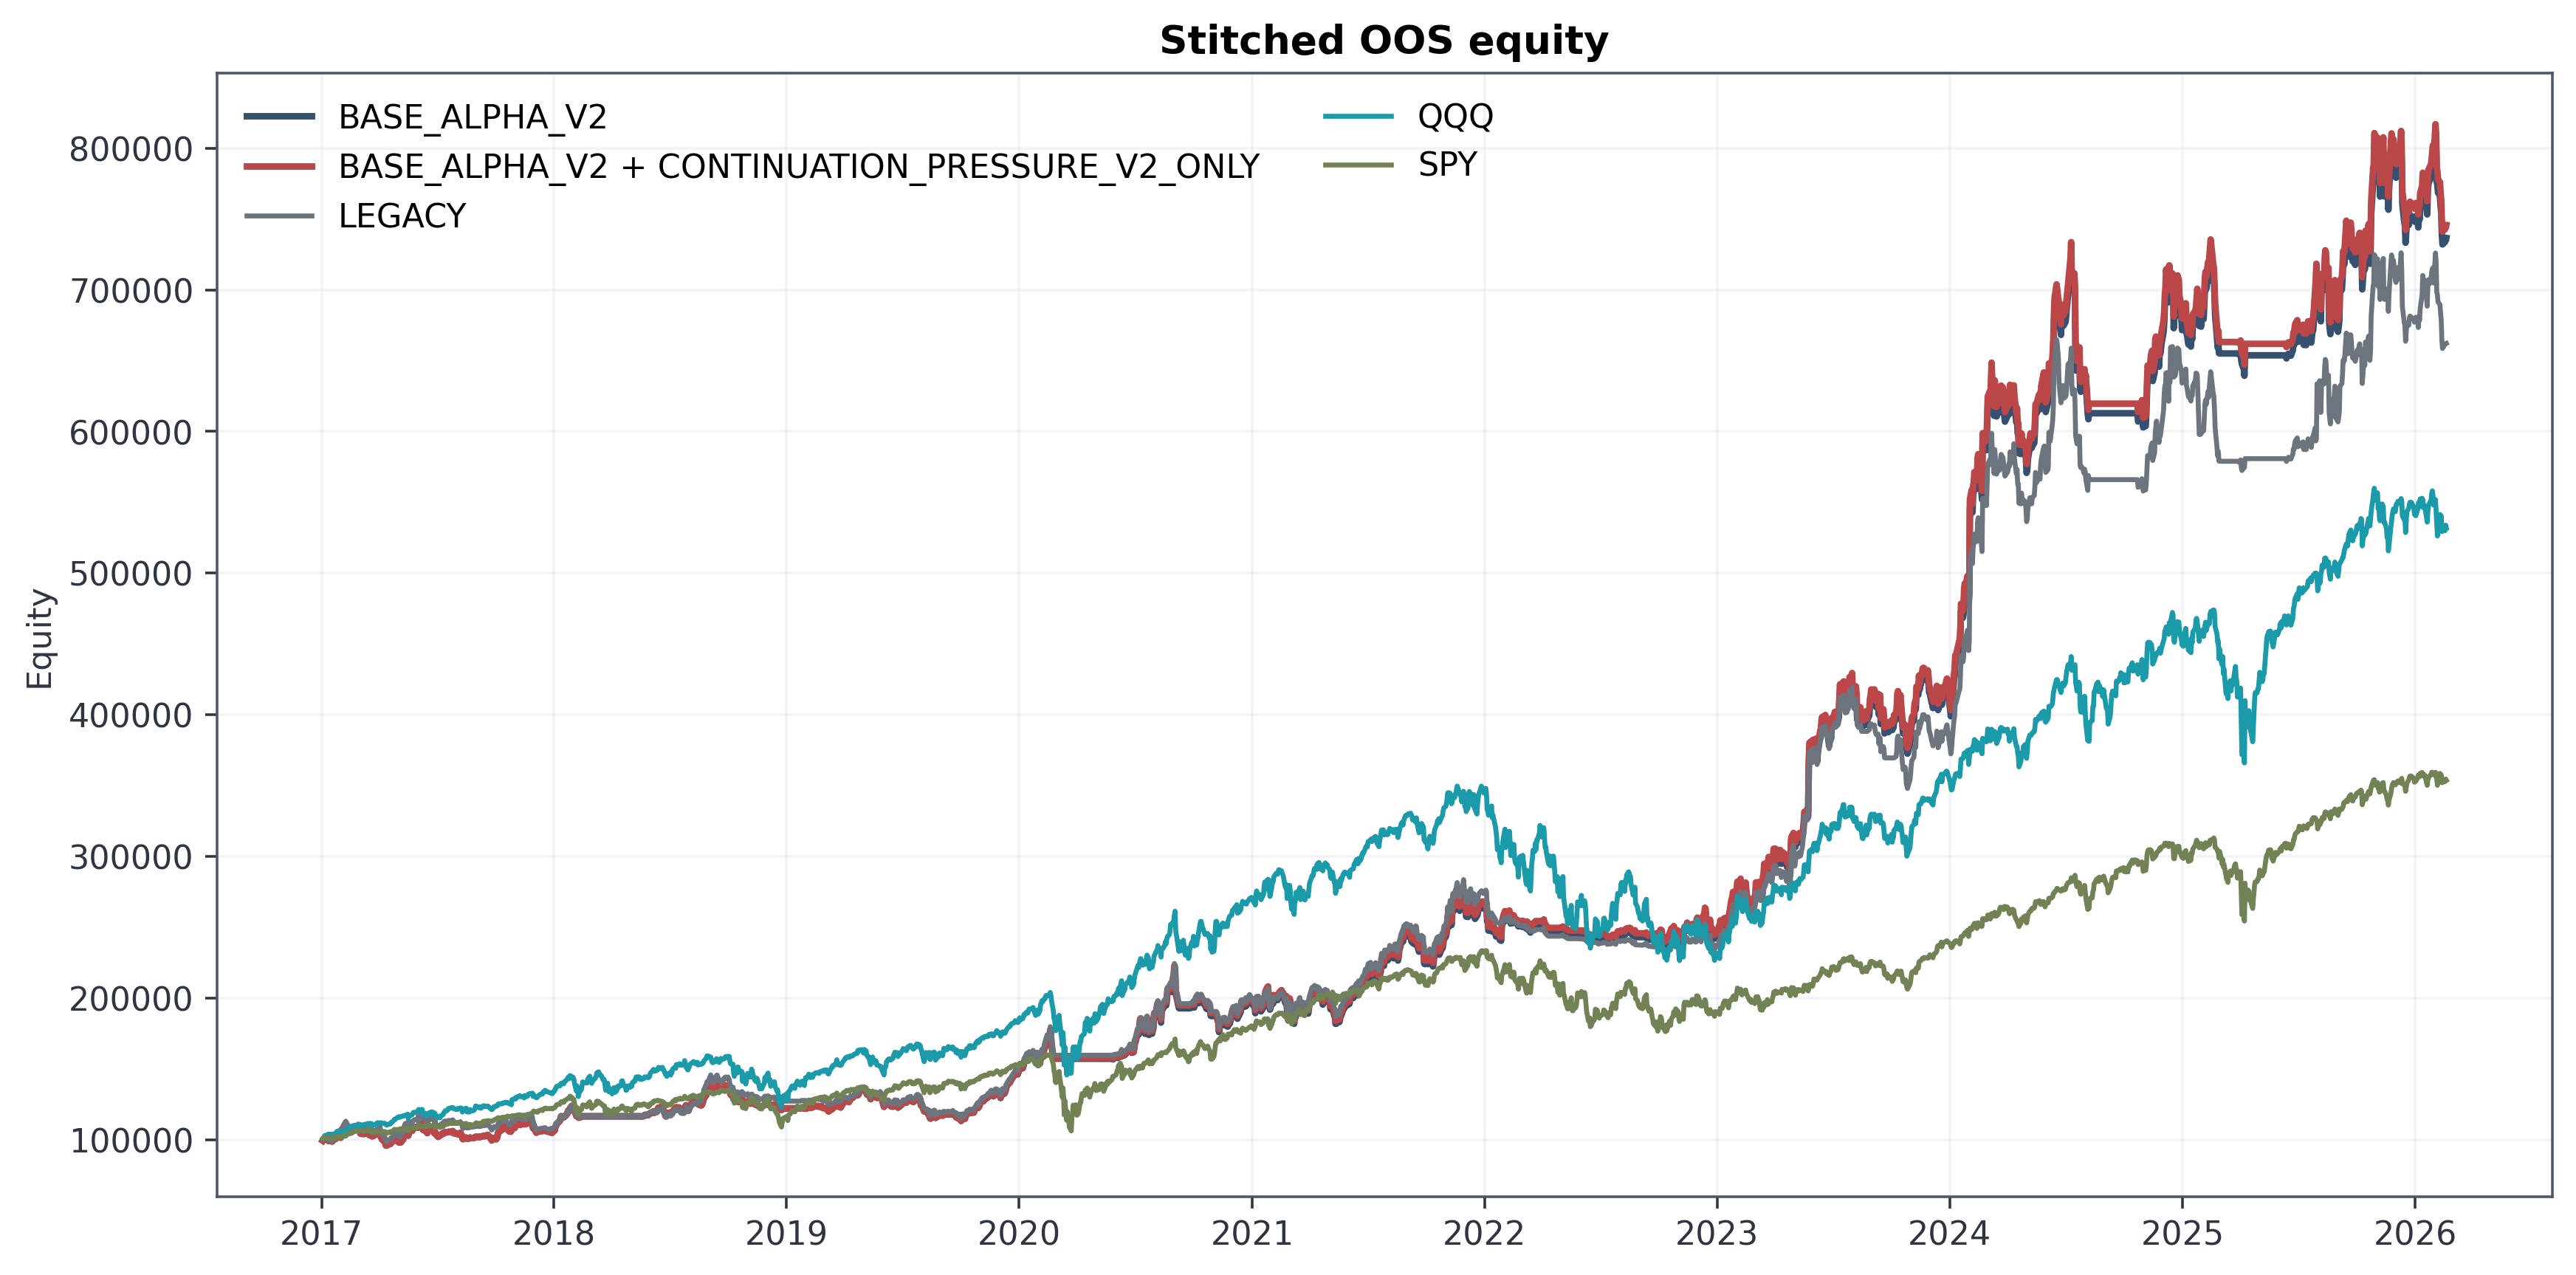
\includegraphics[width=0.92\textwidth]{../mahoraga14_outputs/figures/equity_curve_stitched_full.png}
\caption{Trayectorias de equity stitched para la base, el candidato primario continuation y los benchmarks obligatorios. Archivo fuente: \texttt{equity\_curve\_stitched\_full.png}.}
\label{fig:equity}
\end{figure}

\begin{figure}[H]
\centering
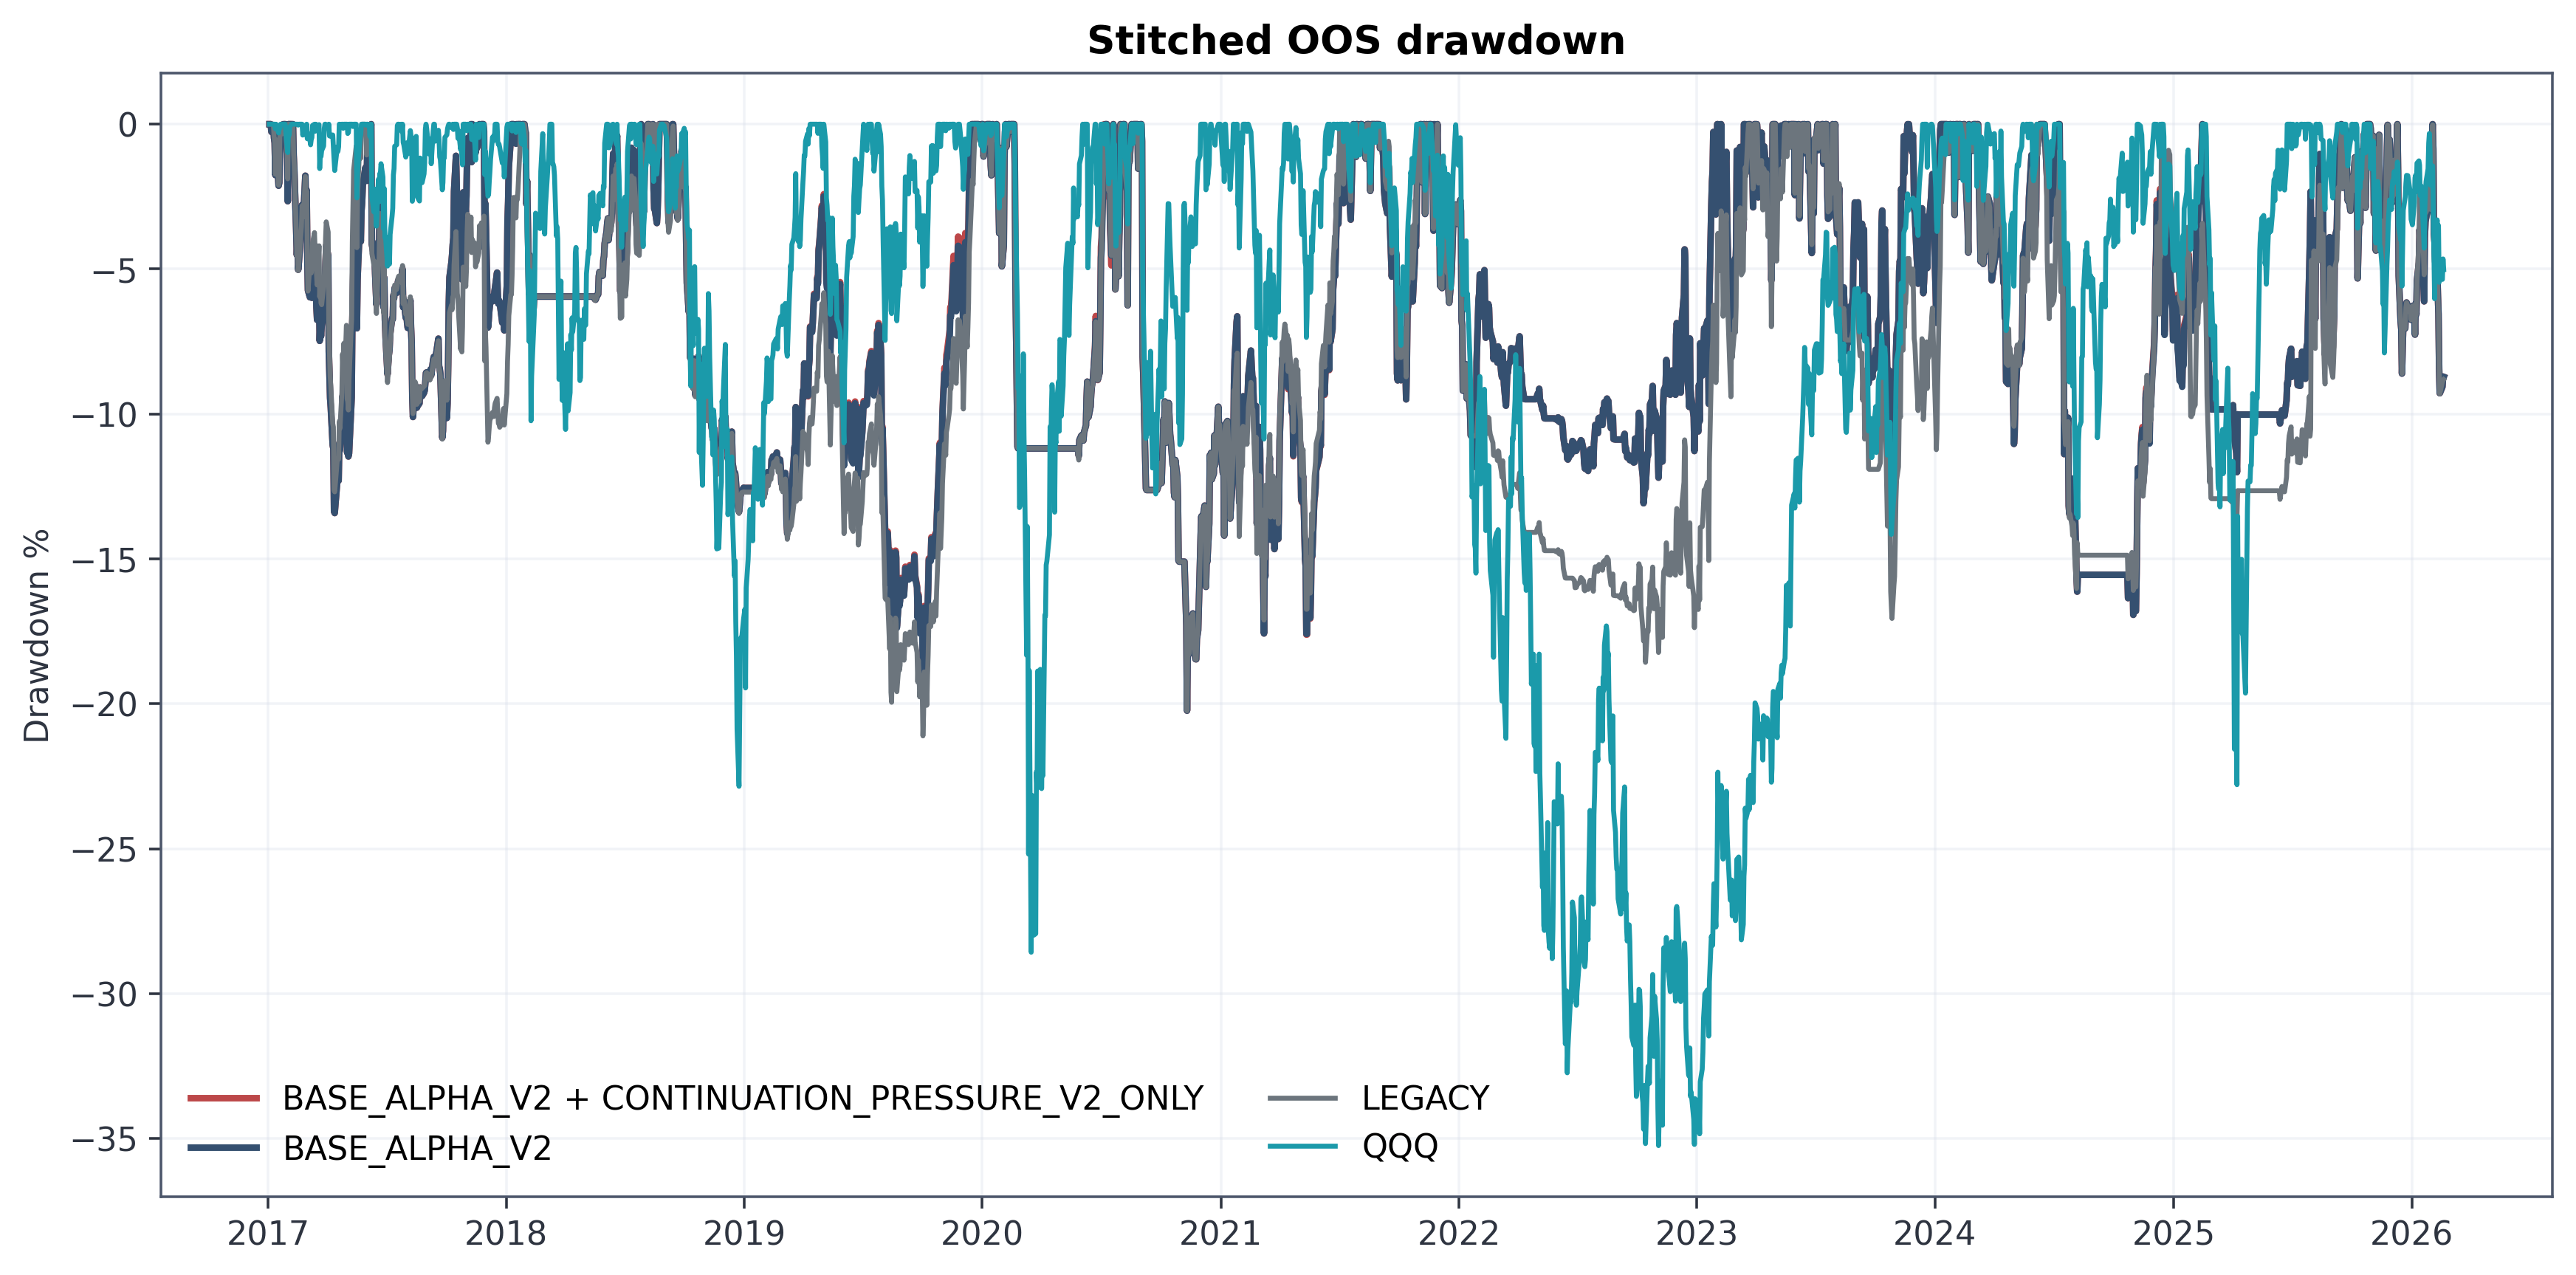
\includegraphics[width=0.92\textwidth]{../mahoraga14_outputs/figures/drawdown_curve_stitched_full.png}
\caption{Curvas stitched de drawdown para el candidato primario, la base, \texttt{LEGACY} y \texttt{QQQ}. Archivo fuente: \texttt{drawdown\_curve\_stitched\_full.png}.}
\label{fig:drawdown}
\end{figure}

\begin{figure}[H]
\centering
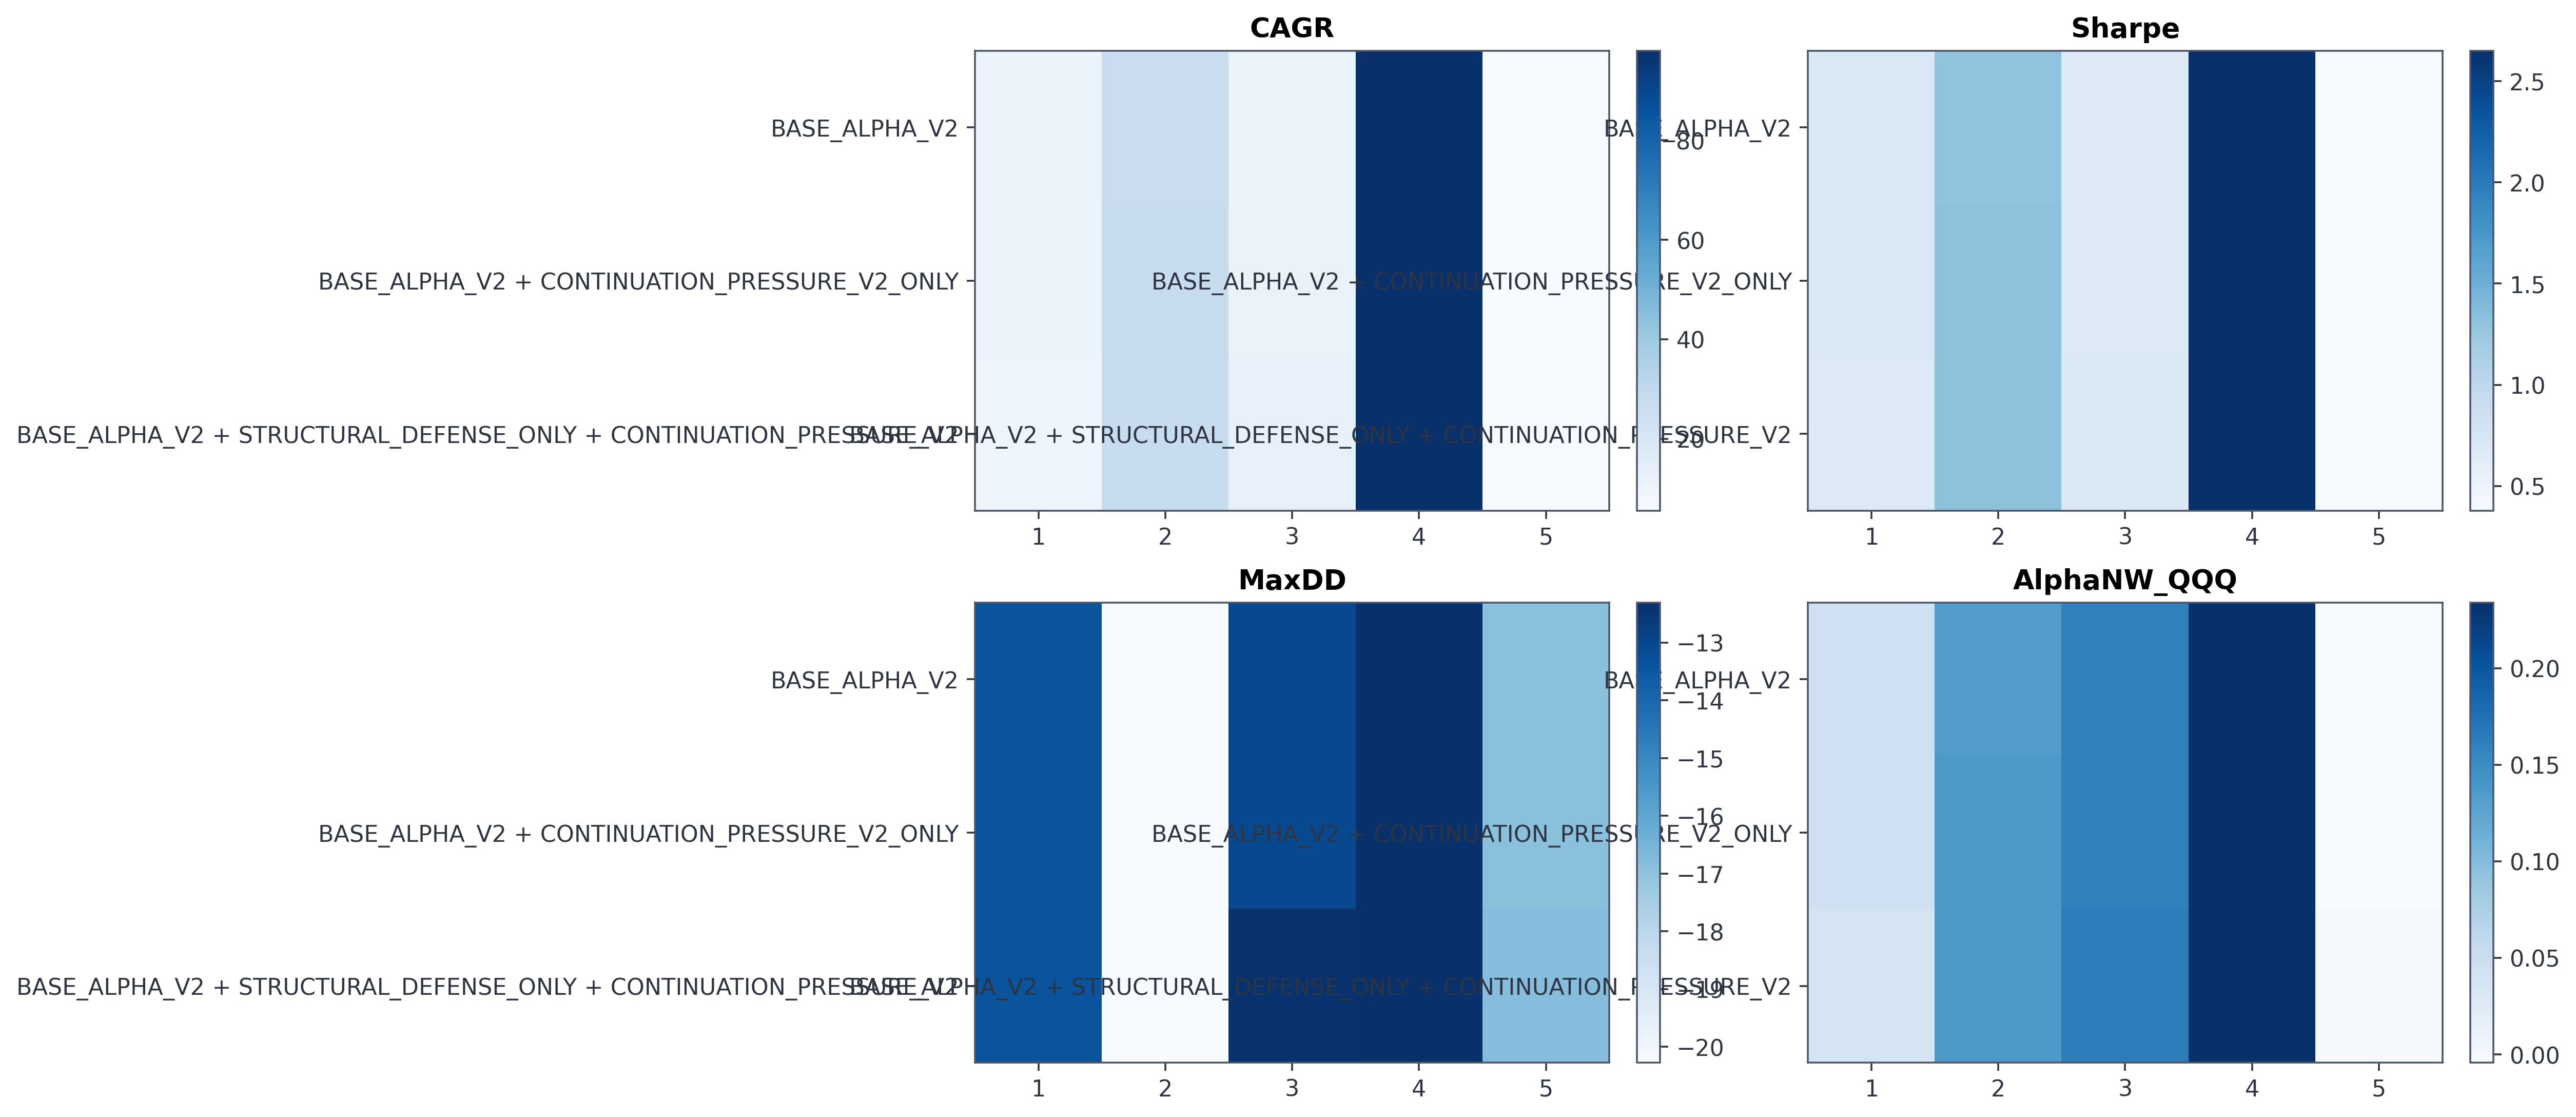
\includegraphics[width=0.92\textwidth]{../mahoraga14_outputs/figures/fold_heatmap_full.png}
\caption{Mapa por fold de CAGR, Sharpe, MaxDD y alpha Newey-West para los candidatos auditados. Archivo fuente: \texttt{fold\_heatmap\_full.png}.}
\label{fig:heatmap}
\end{figure}

\begin{figure}[H]
\centering
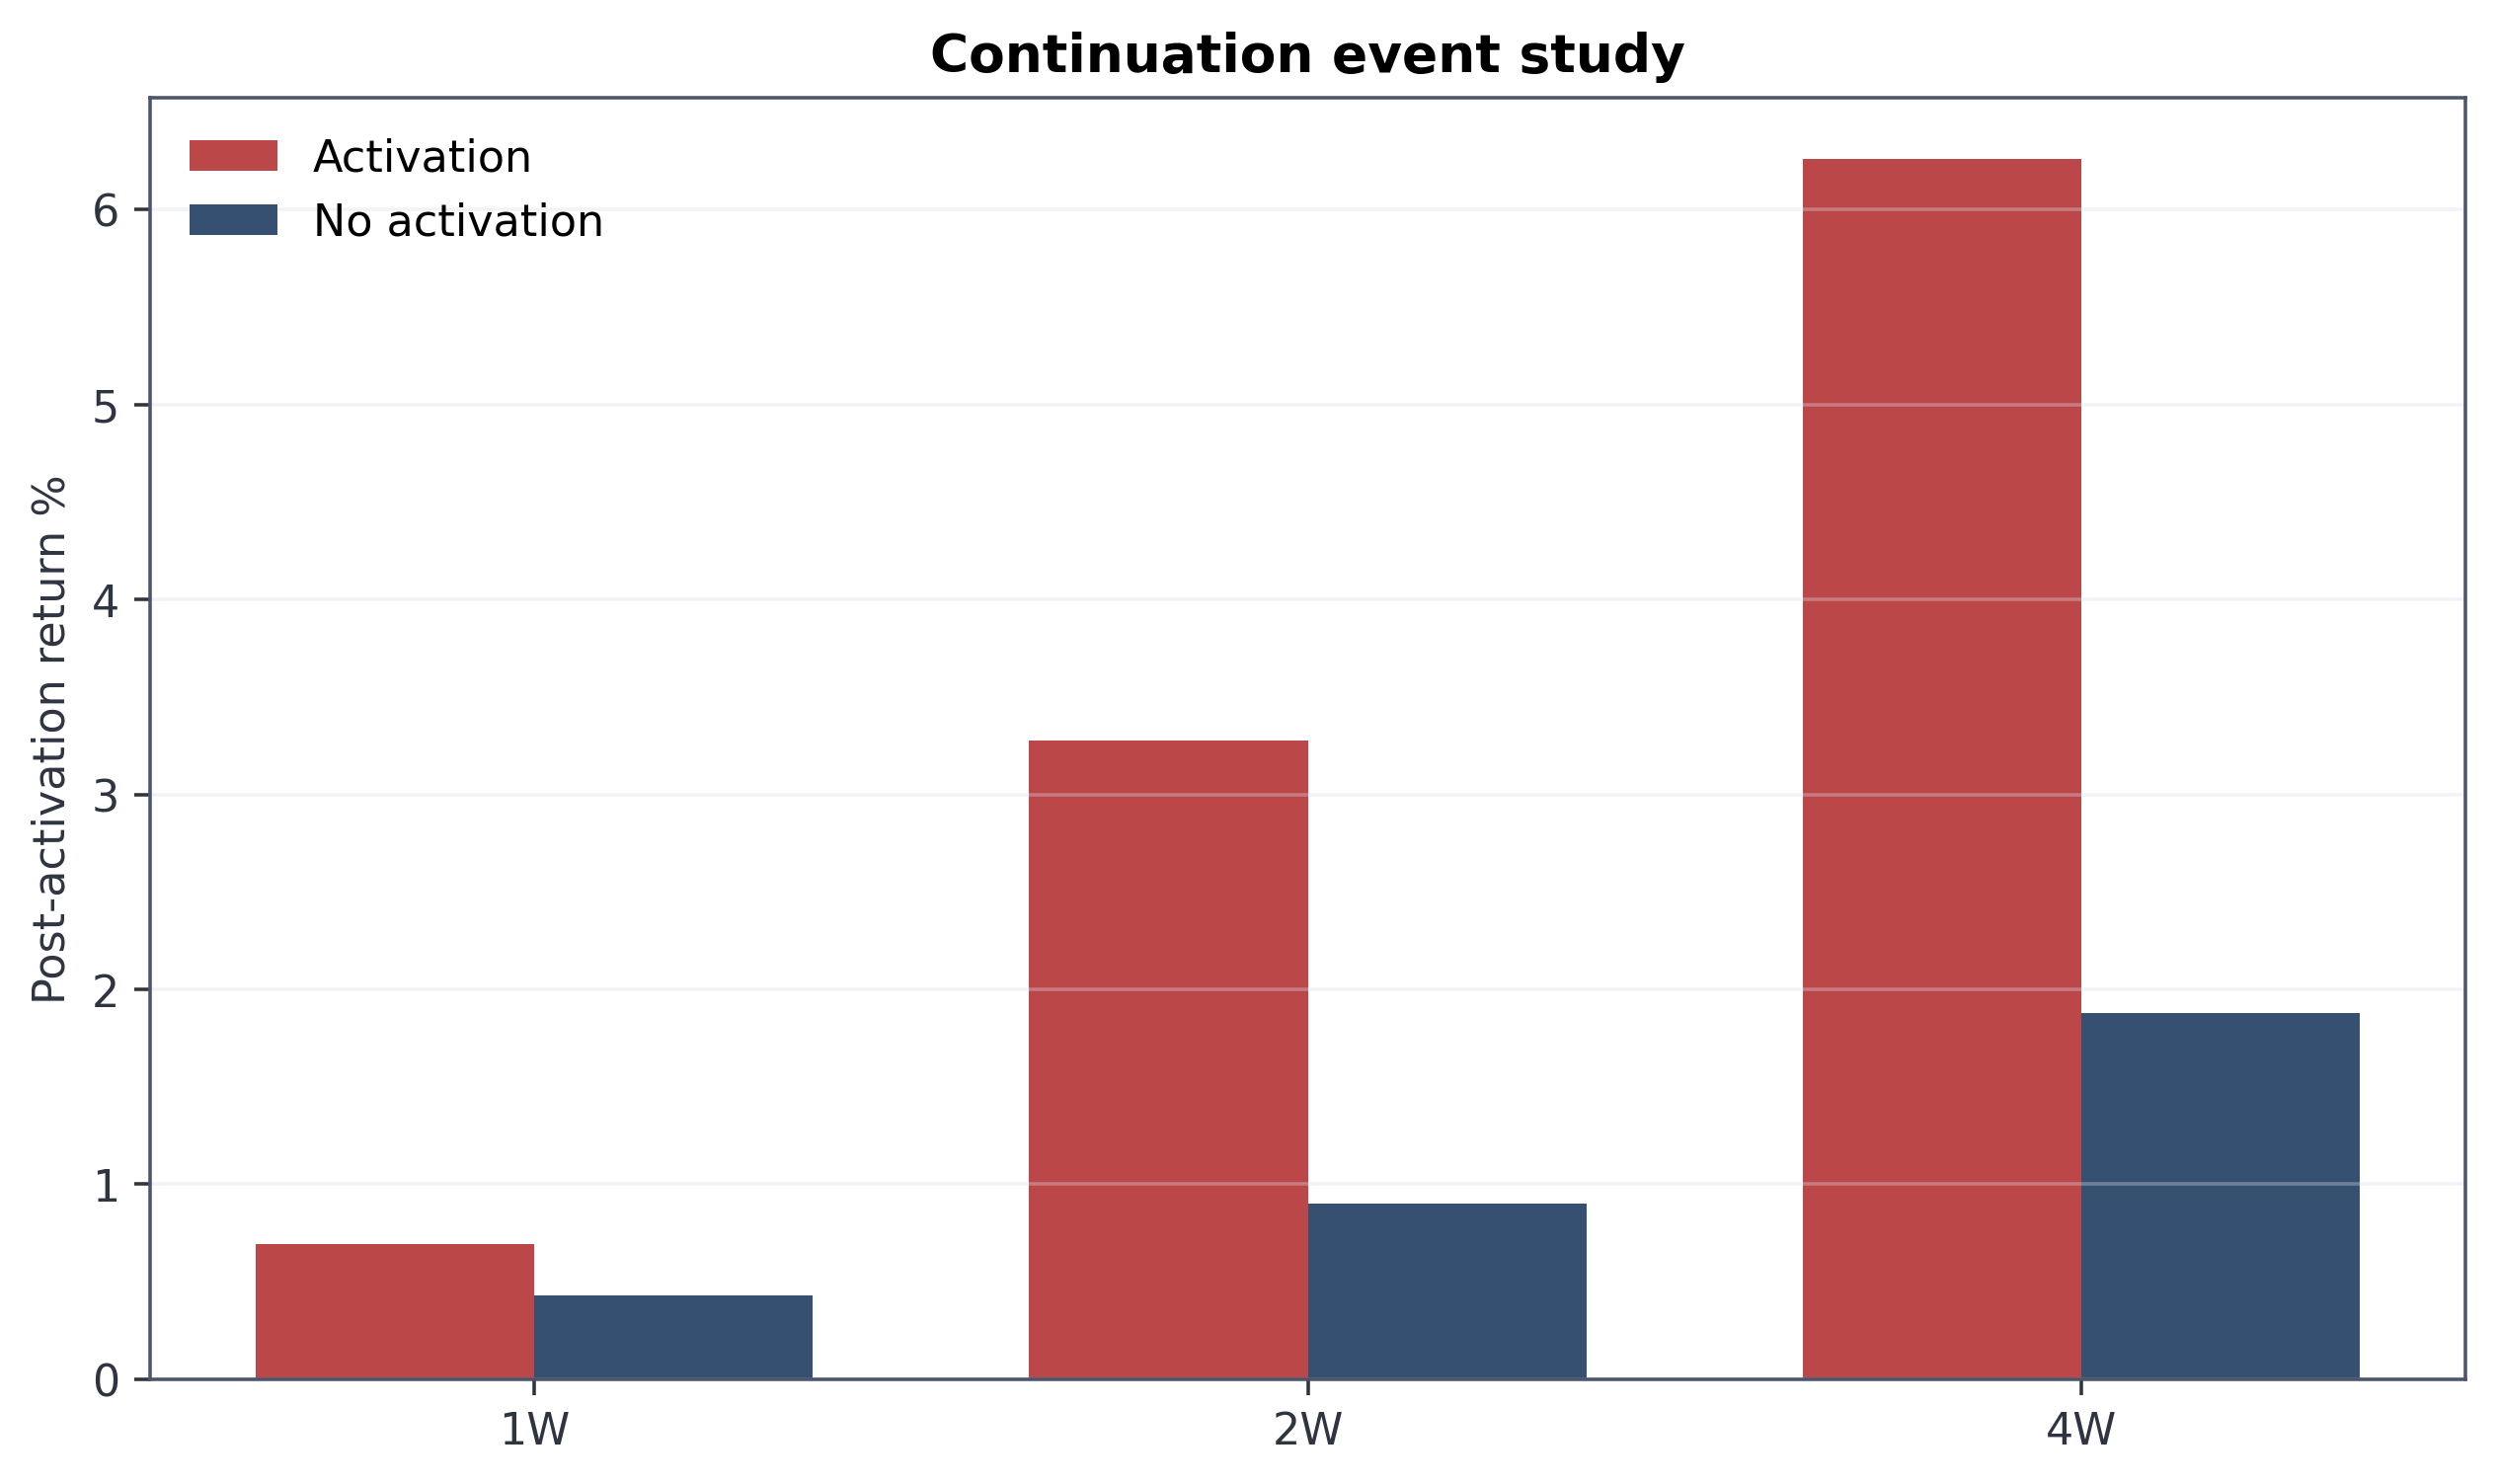
\includegraphics[width=0.82\textwidth]{../mahoraga14_outputs/figures/continuation_event_study_full.png}
\caption{Retornos posteriores a activaciones de continuation frente a semanas sin activaci\'on. Archivo fuente: \texttt{continuation\_event\_study\_full.png}.}
\label{fig:contstudy}
\end{figure}

\begin{figure}[H]
\centering
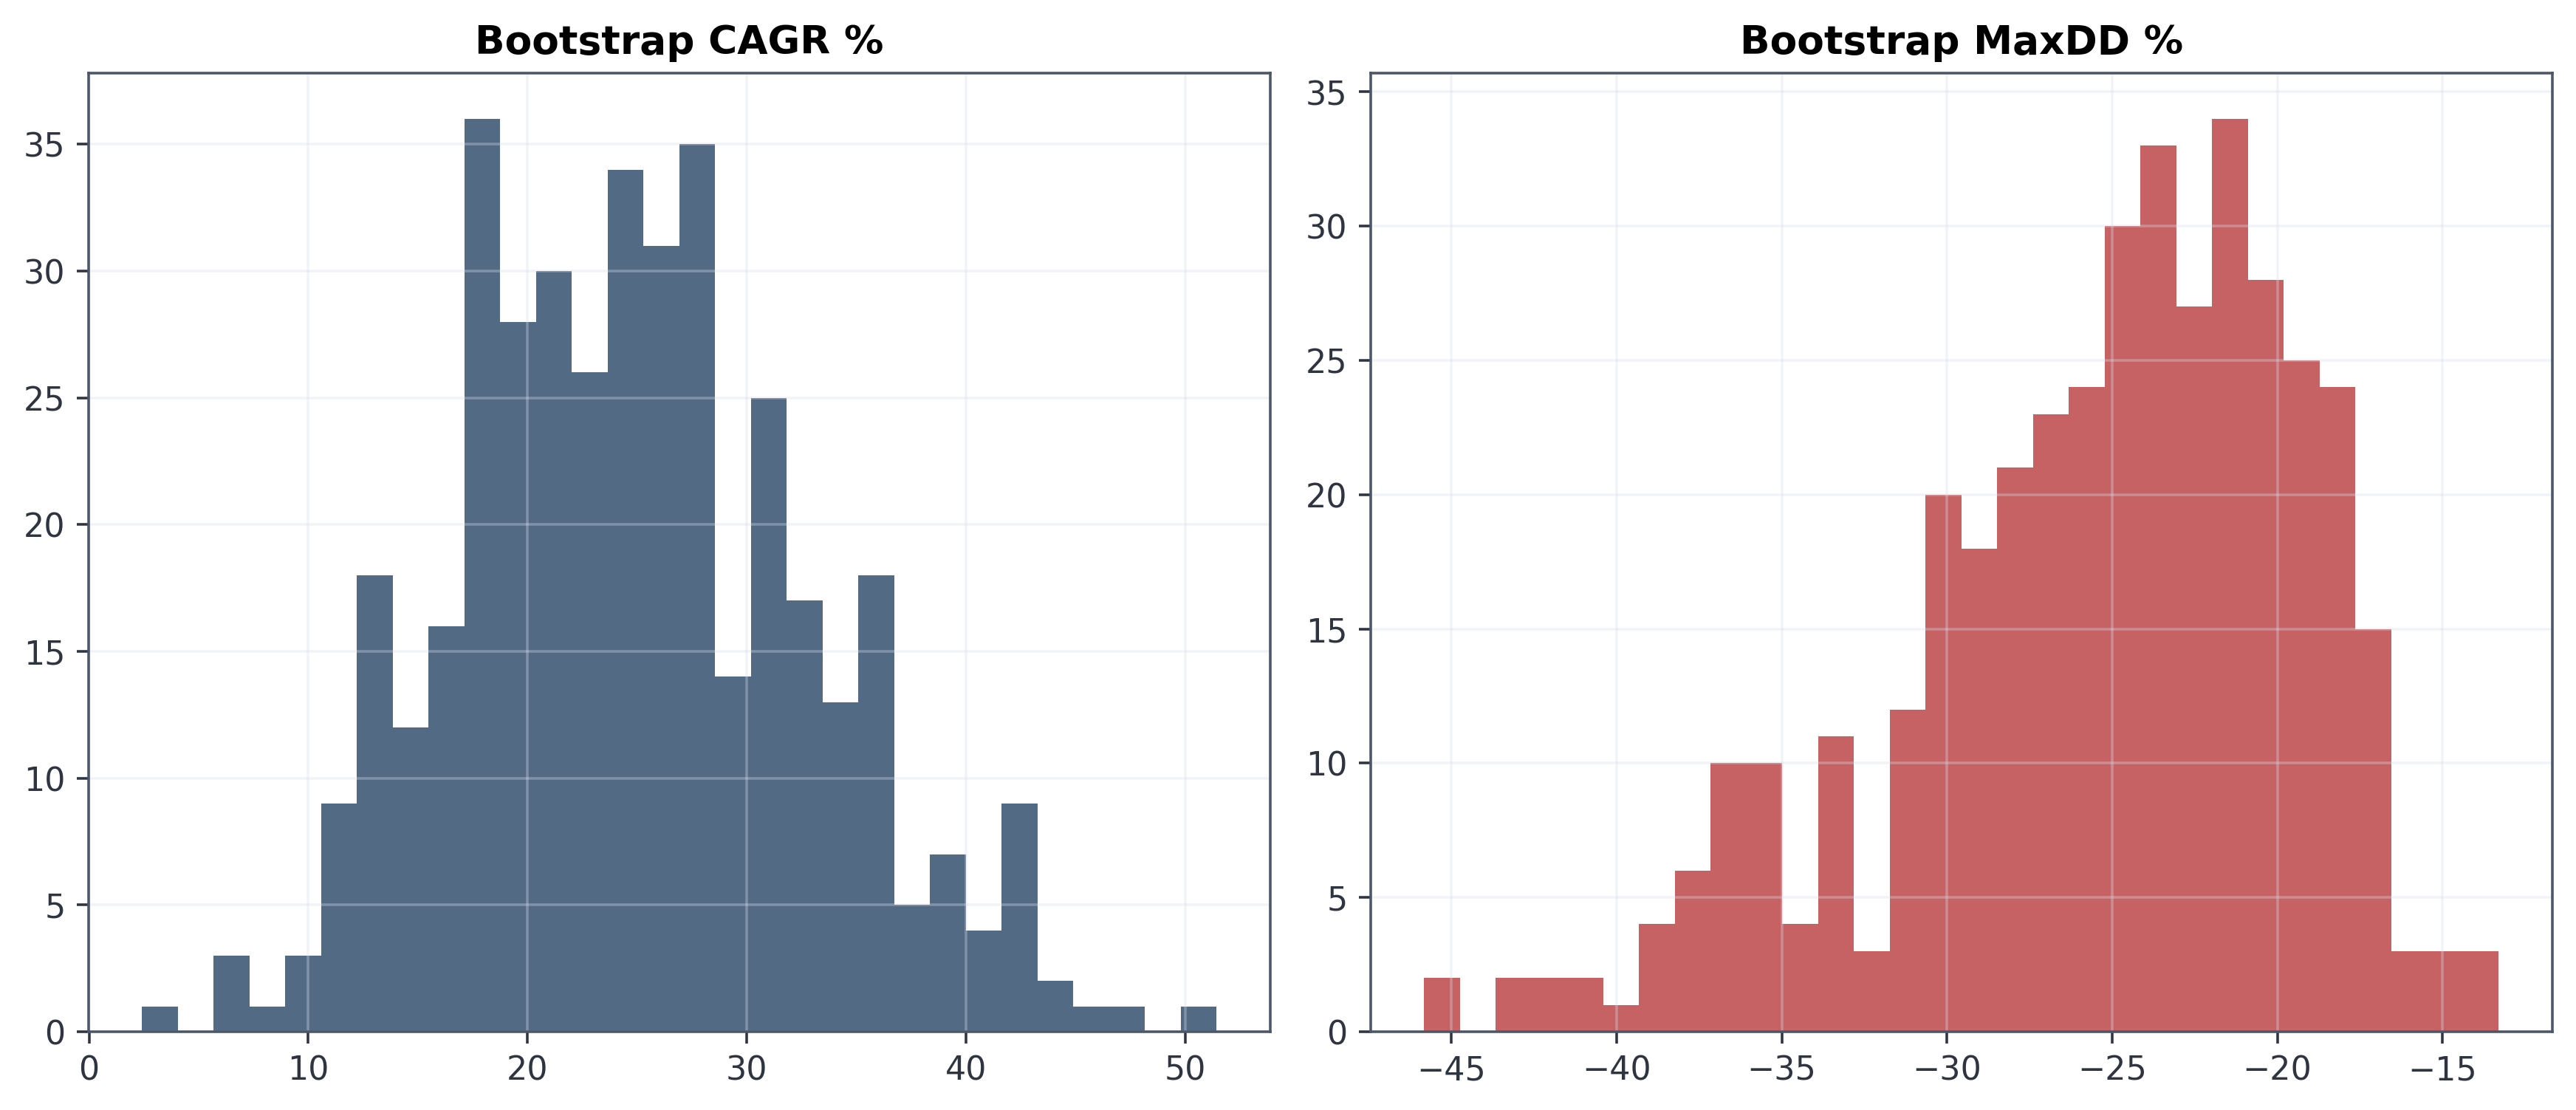
\includegraphics[width=0.82\textwidth]{../mahoraga14_outputs/figures/montecarlo_distribution_full.png}
\caption{Distribuciones Monte Carlo y bootstrap para CAGR y/o MaxDD en las variantes auditadas. Archivo fuente: \texttt{montecarlo\_distribution\_full.png}.}
\label{fig:mc}
\end{figure}

\section{Limitaciones}
La primera limitaci\'on es de universo y datos. Aunque el motor can\'onico es point-in-time respecto al calendario local disponible, el ranking por \textit{LiqSizeProxy} no equivale a FFMC ni a una clasificaci\'on GICS-IT. Por ello, la representaci\'on del universo tecnol\'ogico sigue siendo una aproximaci\'on operativa, no un universo institucional plenamente reproducible con datos CRSP/Compustat.

La segunda limitaci\'on es estad\'istica. La mejora continuation sobre la base existe en stitched agregado, pero es peque\~na y no sobrevive la correcci\'on BHY disponible. En el mismo sentido, el event study stitched de continuation se apoya s\'olo en 10 activaciones, por lo que su lectura debe ser auxiliar y no concluyente.

La tercera limitaci\'on es de robustez. El stationary bootstrap muestra que la distribuci\'on de MaxDD es m\'as adversa que la trayectoria stitched observada. Adem\'as, la suite de stress es razonable y trazable, pero no exhaustiva; en particular, el \textit{empirical tail block path stress} representa una selecci\'on concreta de bloques adversos y no agota todos los reg\'imenes plausibles.

La cuarta limitaci\'on es de alcance del paper. Este trabajo describe exclusivamente la implementaci\'on operativa de Mahoraga 14.1 y sus salidas FULL auditadas. No debe leerse como validaci\'on de m\'odulos presentes en el repositorio pero inactivos en la ruta de ejecuci\'on final.

\section{Conclusiones}
Mahoraga 14.1 puede caracterizarse con precisi\'on como una consolidaci\'on auditada de Mahoraga 14. El aporte principal no es una nueva arquitectura, sino la depuraci\'on metodol\'ogica del modo FULL. La auditor\'ia confirma que el stitched OOS concatena exclusivamente ventanas \texttt{TEST\_ONLY}, que el MaxDD stitched coincide exactamente con una recomputaci\'on independiente y que la suite de stress y Monte Carlo opera sobre la serie correcta sin romper la dependencia temporal de forma ingenua.

En t\'erminos de desempe\~no, \texttt{BASE\_ALPHA\_V2} sigue siendo la base fuerte. La rama continuation aporta una mejora stitched peque\~na pero real y se convierte en el candidato primario auditado de 14.1. La defensa estructural conserva valor como m\'odulo de apoyo al suelo y como componente del combo, pero no como rama principal agregada. El alpha benchmark-adjusted frente a \texttt{QQQ} y \texttt{SPY} permanece positivo, mientras que la comparaci\'on directa continuation vs.\ base exige moderaci\'on por su fragilidad bajo correcci\'on por multiplicidad.

En conjunto, la evidencia disponible respalda que Mahoraga 14.1 ya no debe evaluarse como un prototipo ambiguo de investigaci\'on, sino como una implementaci\'on auditable y coherente con FAST. Esa conclusi\'on es suficientemente fuerte para documentaci\'on t\'ecnica y an\'alisis formal, pero no autoriza exagerar la magnitud del edge ni ocultar los riesgos abiertos de universo, tama\~no muestral y sensibilidad de cola.

\section*{References}
\begin{thebibliography}{99}

\bibitem{Breiman2001}
Breiman, L. (2001). Random forests. \textit{Machine Learning, 45}(1), 5--32.

\bibitem{Hawkes1971}
Hawkes, A. G. (1971). Spectra of some self-exciting and mutually exciting point processes. \textit{Biometrika, 58}(1), 83--90.

\bibitem{HoerlKennard1970}
Hoerl, A. E., \& Kennard, R. W. (1970). Ridge regression: Biased estimation for nonorthogonal problems. \textit{Technometrics, 12}(1), 55--67.

\bibitem{LopezdePrado2016}
L\'opez de Prado, M. (2016). Building diversified portfolios that outperform out of sample. \textit{The Journal of Portfolio Management, 42}(4), 59--69.

\bibitem{NeweyWest1987}
Newey, W. K., \& West, K. D. (1987). A simple, positive semi-definite, heteroskedasticity and autocorrelation consistent covariance matrix. \textit{Econometrica, 55}(3), 703--708.

\end{thebibliography}

\end{document}
